\documentclass{beamer}
\usepackage[utf8]{inputenc}
\usepackage{graphicx, epsfig}
\usepackage{amsmath,mathrsfs,amsfonts,amssymb}
%\usepackage{subfig}
\usepackage{floatflt}
\usepackage{epic,ecltree}
\usepackage{mathtext}
\usepackage{fancybox}
\usepackage{fancyhdr}
\usepackage{multirow}
\usepackage{enumerate}
\usepackage{epstopdf}
\usepackage{multicol}
\usepackage{algorithm}
\usepackage[noend]{algorithmic}
\def\algorithmicrequire{\textbf{Input:}}
\def\algorithmicensure{\textbf{Output:}}
\usetheme{default}%{Singapore}%{Warsaw}%{Warsaw}%{Darmstadt}
\usecolortheme{default}
\setbeamerfont{title}{size=\Huge}
\setbeamertemplate{footline}[page number]{}
\setbeamerfont{title}{size=\Huge}
\beamertemplatenavigationsymbolsempty

% latin bold lower
\newcommand{\ba}{\mathbf{a}} 
\newcommand{\bc}{\mathbf{c}} 
\newcommand{\be}{\mathbf{e}} 
\newcommand{\bh}{\mathbf{h}} 
\newcommand{\bp}{\mathbf{p}} 
\newcommand{\bt}{\mathbf{t}} 
\newcommand{\bu}{\mathbf{u}} 
\newcommand{\bv}{\mathbf{v}} 
\newcommand{\bw}{\mathbf{w}} 
\newcommand{\bx}{\mathbf{x}} 
\newcommand{\by}{\mathbf{y}} 
\newcommand{\bz}{\mathbf{z}} 

% latin bold upper
\newcommand{\bA}{\mathbf{A}} 
\newcommand{\bC}{\mathbf{C}} 
\newcommand{\bI}{\mathbf{I}} 
\newcommand{\bM}{\mathbf{M}} 
\newcommand{\bT}{\mathbf{T}} 
\newcommand{\bU}{\mathbf{U}} 
\newcommand{\bW}{\mathbf{W}} 
\newcommand{\bX}{\mathbf{X}} 
\newcommand{\bY}{\mathbf{Y}} 
\newcommand{\bZ}{\mathbf{Z}} 

% latin cal upper
\newcommand{\cL}{\mathcal{L}} 
\newcommand{\cN}{\mathcal{N}} 
\newcommand{\cS}{\mathcal{S}} 
\newcommand{\cT}{\mathcal{T}} 
\newcommand{\cW}{\mathcal{W}} 
\newcommand{\cX}{\mathcal{X}} 
\newcommand{\cZ}{\mathcal{Z}} 

% latin cal upper
\newcommand{\bbE}{\mathbb{E}} 
\newcommand{\bbP}{\mathbb{P}} 
\newcommand{\bbR}{\mathbb{R}} 

% greek bold lower
\newcommand{\bepsilon}{\boldsymbol{\epsilon}} 
\newcommand{\btheta}{\boldsymbol{\theta}} 
\newcommand{\blambda}{\boldsymbol{\lambda}} 
\newcommand{\bmu}{\boldsymbol{\mu}} 
\newcommand{\bsigma}{\boldsymbol{\sigma}} 
\newcommand{\bphi}{\boldsymbol{\phi}} 

% greek bold upper
\newcommand{\bSigma}{\boldsymbol{\Sigma}} 

\DeclareMathOperator*{\argmin}{arg\,min}
\DeclareMathOperator*{\argmax}{arg\,max}

\newcommand{\createdgmtitle}[1]{\title[\hbox to 56mm{Deep Generative Models  \hfill\insertframenumber\,/\,\inserttotalframenumber}]
	{\vspace{1cm} \\ Deep Generative Models \\ Lecture #1 \\ \vspace{-0.5cm}}
	\author{Roman Isachenko \\ \vspace{-0.5cm}}
	\institute{
\includegraphics[width=3cm]{../utils/ozonmasterslogo}
	\\Ozon Masters
	}
	\date{Spring, 2021}
}

\newcommand\myfootnote[1]{%
  \tikz[remember picture,overlay]
  \draw (current page.south west) +(1in + \oddsidemargin,0.5em)
  node[anchor=south west,inner sep=0pt]{\parbox{\textwidth}{%
      \rlap{\rule{10em}{0.4pt}}\raggedright\scriptsize#1}};}

\newcommand\myfootnotewithlink[2]{%
  \tikz[remember picture,overlay]
  \draw (current page.south west) +(1in + \oddsidemargin,0.5em)
  node[anchor=south west,inner sep=0pt]{\parbox{\textwidth}{%
      \rlap{\rule{10em}{0.4pt}}\raggedright\scriptsize\href{#1}{\textit{#2}}}};}
\createdgmtitle{1}
%--------------------------------------------------------------------------------
\begin{document}
%--------------------------------------------------------------------------------
\begin{frame}
%\thispagestyle{empty}
\titlepage
\end{frame}
%--------------------------------------------------------------------------------
\section{Logistics}
%=======
\begin{frame}{Logistics}
    \begin{itemize}
        \item homeworks: 30 points
        \begin{itemize}
            \item hw1: autoregressive models
            \item hw2: latent variable models
            \item hw3: flow models
            \item hw4: adversarial models
        \end{itemize}
        \item exam: 30 points
        \item final project: 40 points
    \end{itemize}
    Last year course page: \href{http://bit.ly/IS_B2}{link} \\
    Admission: \href{https://docs.google.com/spreadsheets/d/1FpTneCfkYNIG1FMxG7ALTwMCGDngkqc_OJC6SDqeG0Q/edit?usp=sharing}{link}
\end{frame}
%--------------------------------------------------------------------------------
\section{Intro}
%=======
\begin{frame}{Generative models zoo}
    \begin{figure}
        \centering
        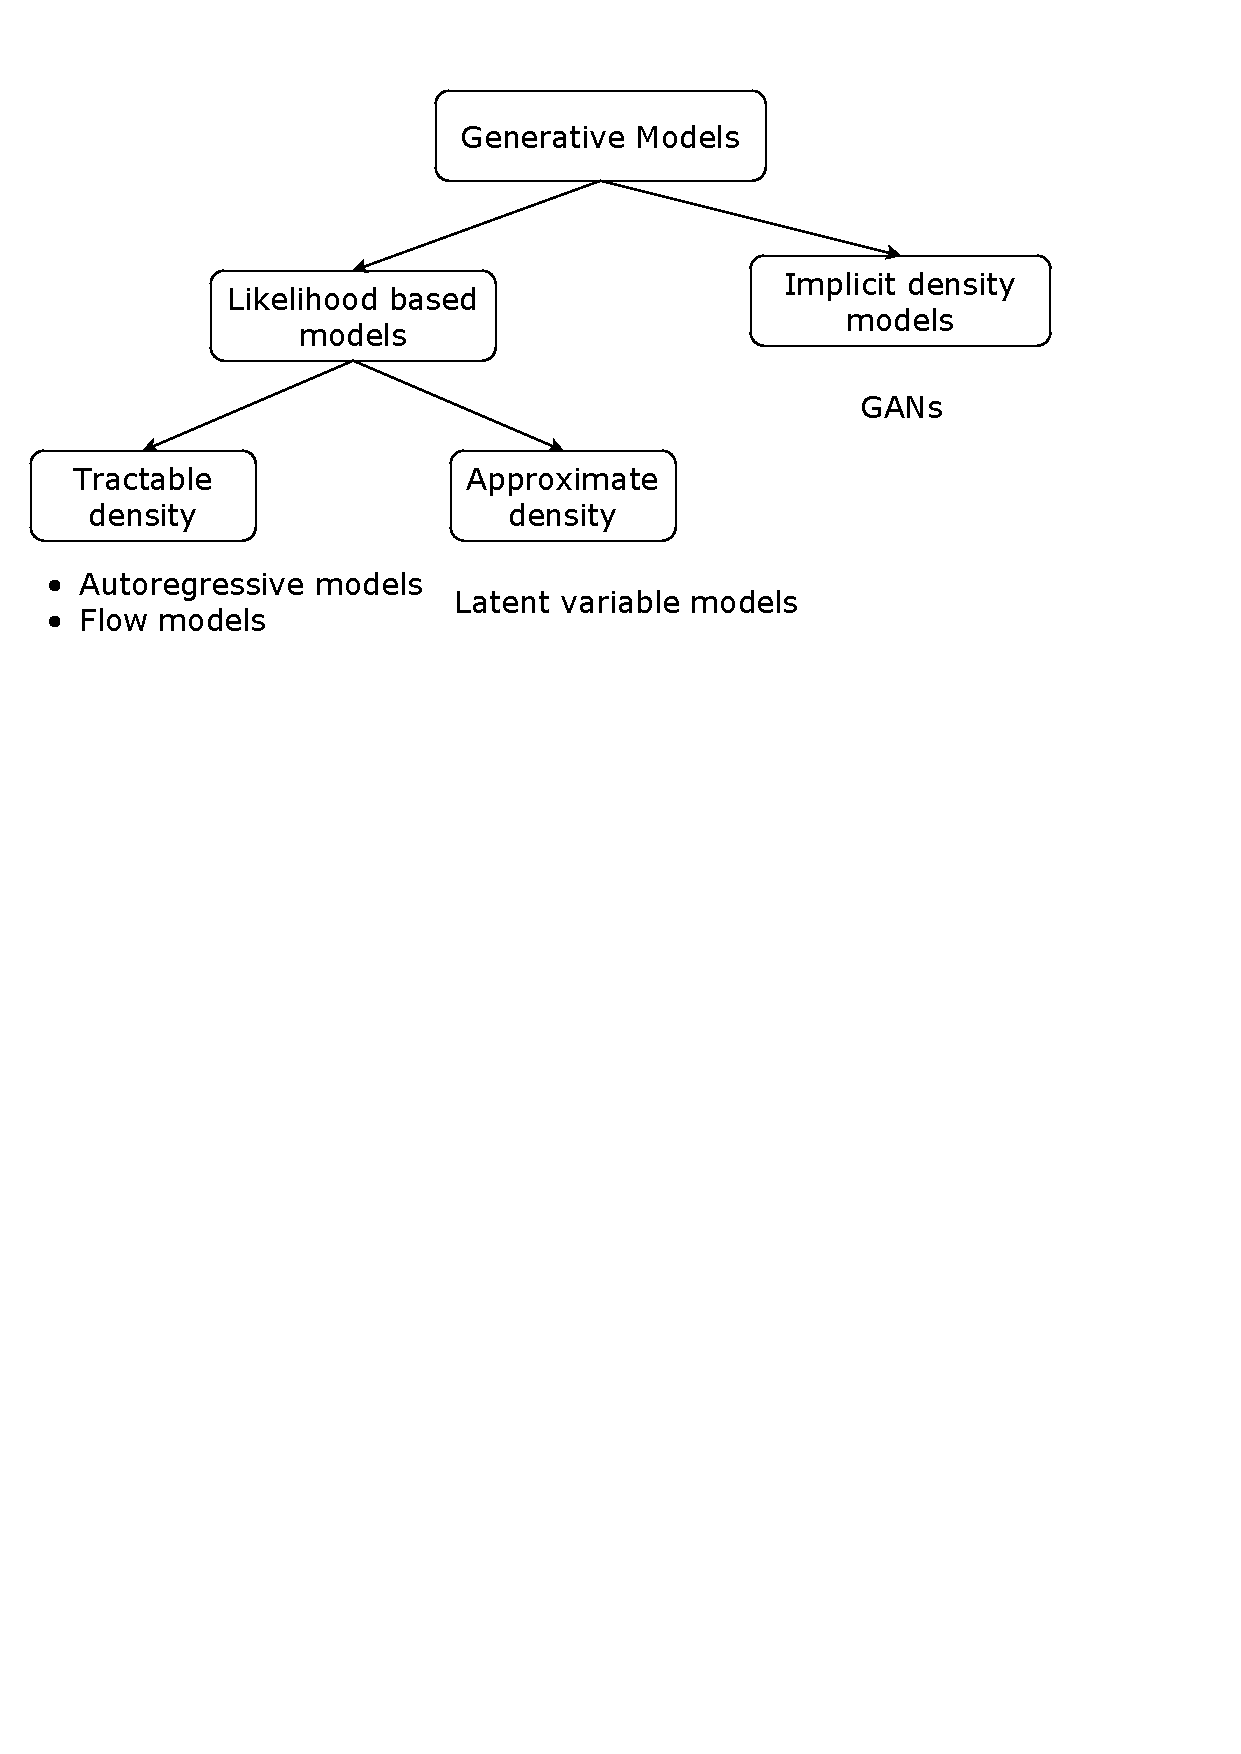
\includegraphics[width=1.0\linewidth]{figs/generative_models_zoo.pdf}
        \label{fig:generative_models_zoo}
    \end{figure}
\end{frame}
\begin{frame}{Motivation}
    \begin{figure}
        \centering
        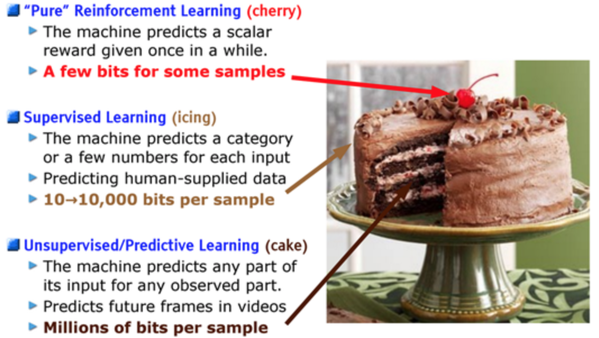
\includegraphics[width=\linewidth]{figs/unsupervised_cake.png}
        \label{fig:unsupervised_cake}
    \end{figure}
\myfootnote{LeCun, NIPS 2016 Keynote}
\end{frame}
%=======
\begin{frame}{Applications: Image generation (VAE)}
    \begin{figure}
        \centering
        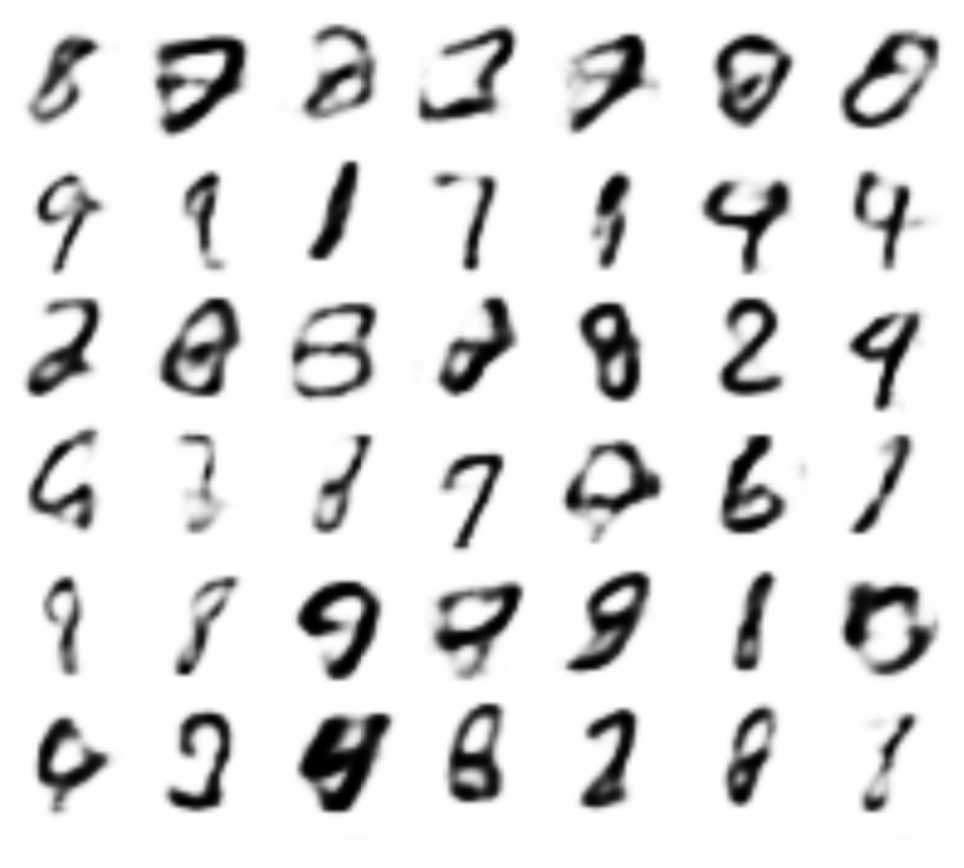
\includegraphics[width=0.5\linewidth]{figs/vae.png}
        \label{fig:vae}
    \end{figure}
\myfootnotewithlink{https://arxiv.org/abs/1312.6114}{Kingma D. P., Welling M. Auto-encoding variational bayes, 2013}
\end{frame}
%=======
\begin{frame}{Applications: Image generation (DCGAN)}
    \begin{figure}
        \centering
        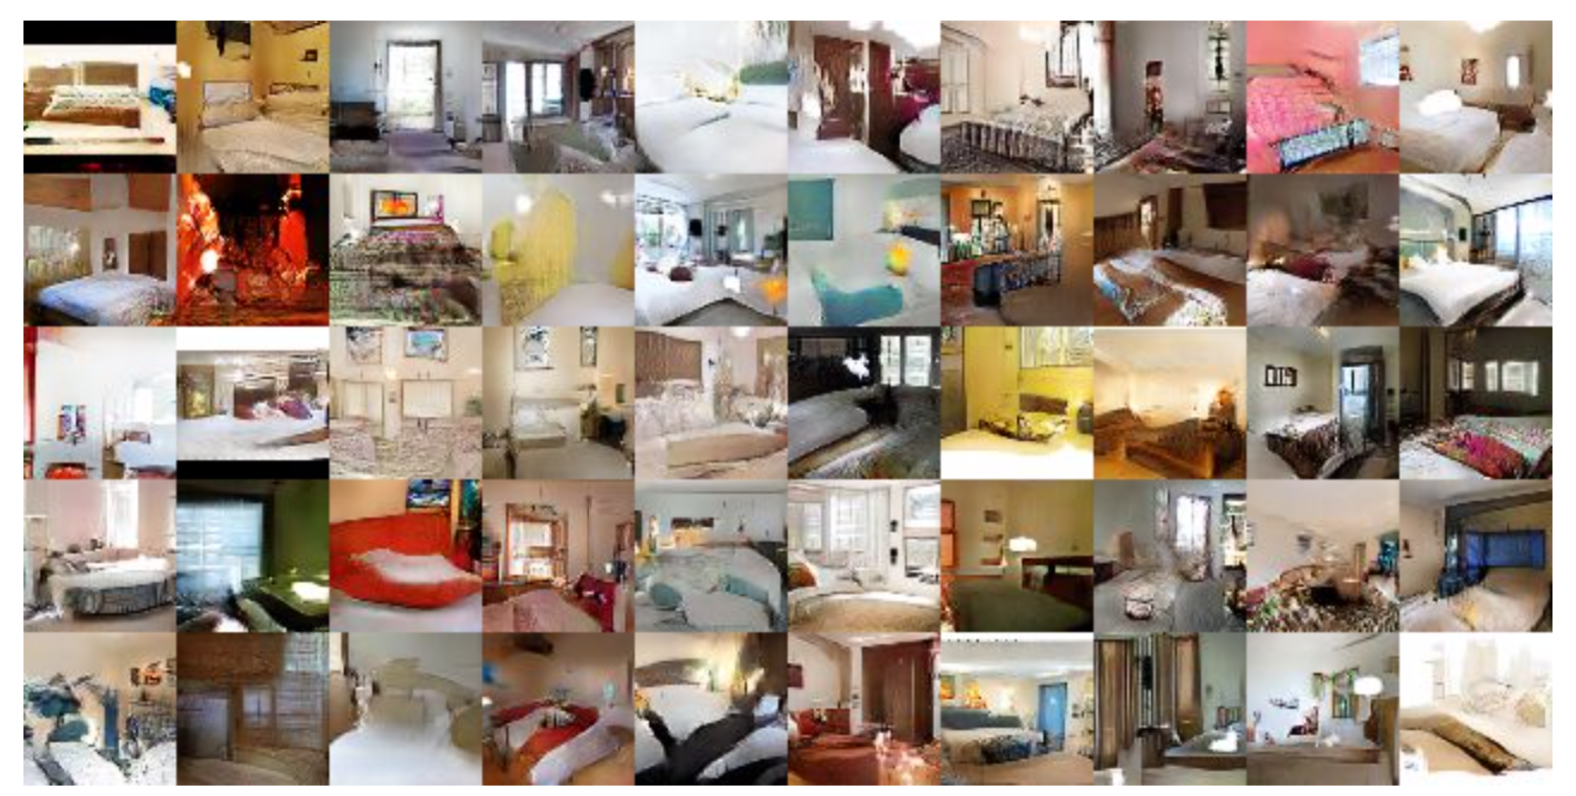
\includegraphics[width=1.0\linewidth]{figs/dcgan.png}
        \label{fig:dcgan}
    \end{figure}
\myfootnotewithlink{https://arxiv.org/abs/1511.06434}{Radford A., Metz L., Chintala S. Unsupervised representation learning with deep convolutional generative adversarial networks, 2015}
\end{frame}
%=======
\begin{frame}{Applications: SuperResolution (SRGAN)}
    \begin{figure}
        \centering
        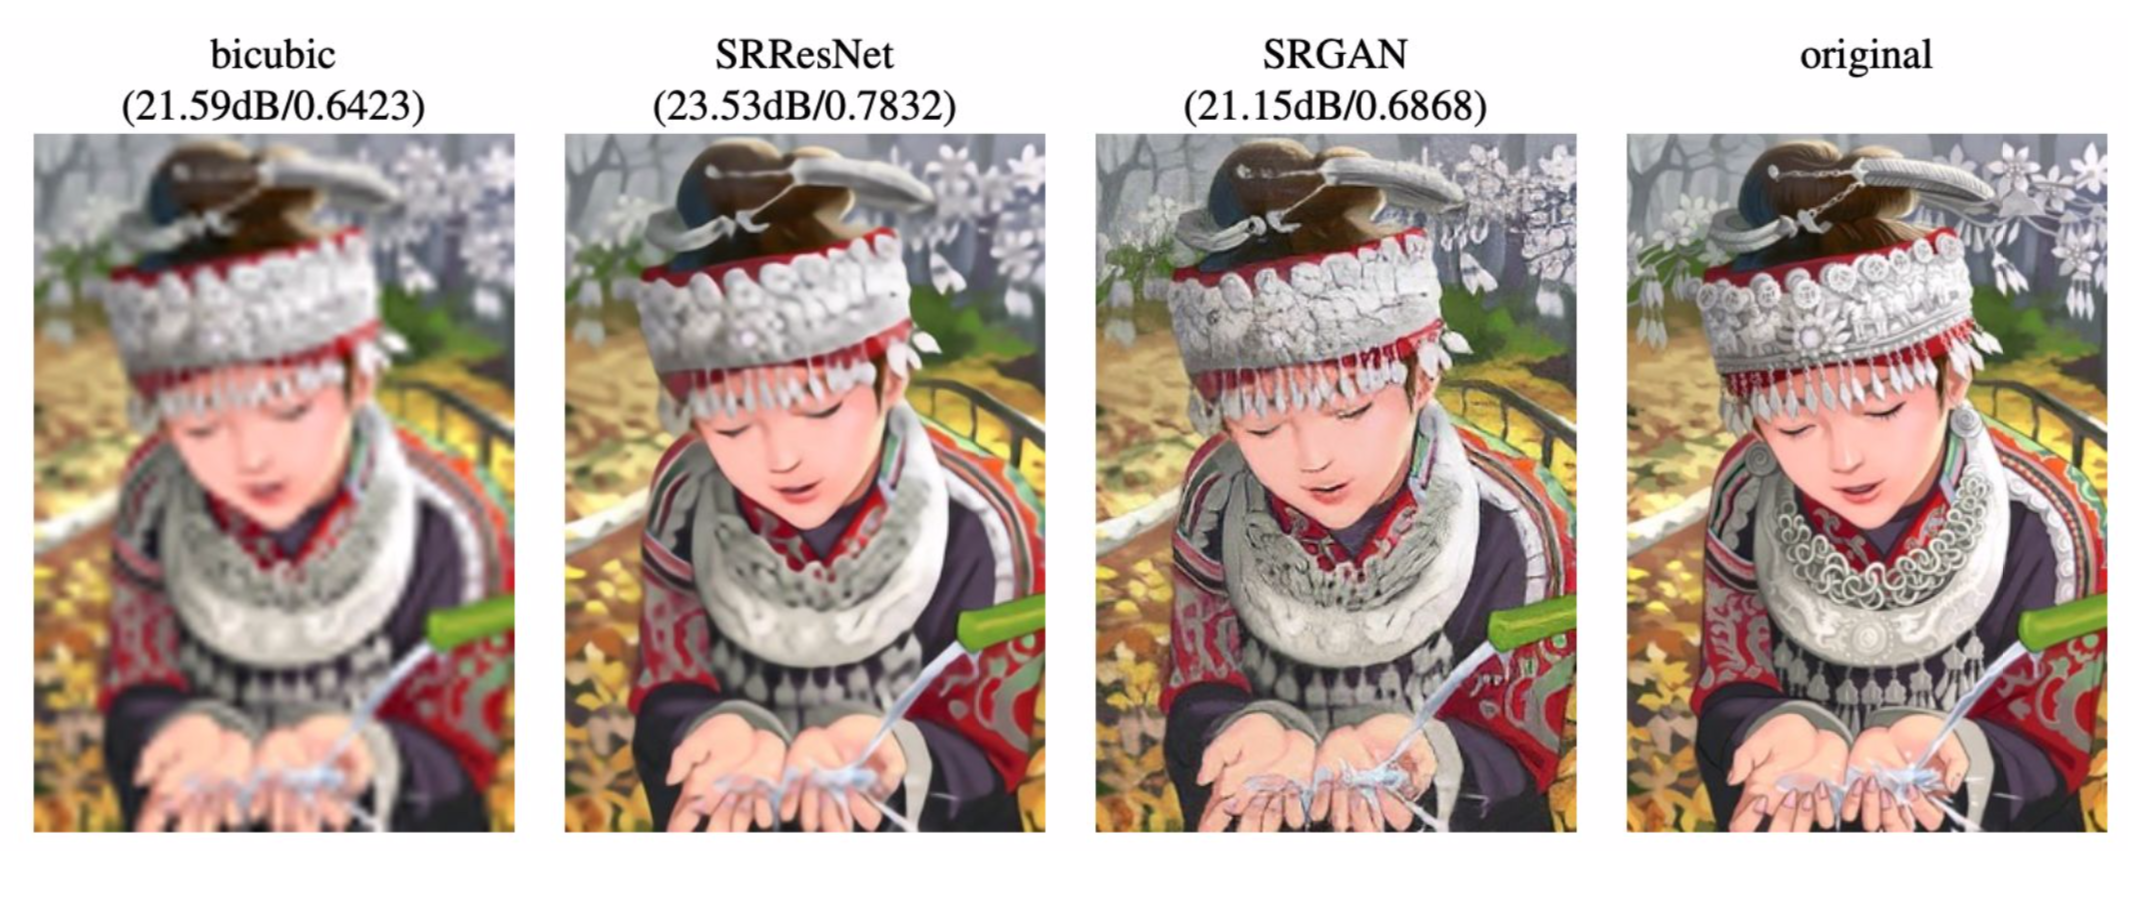
\includegraphics[width=1.0\linewidth]{figs/srgan.png}
        \label{fig:srgan}
    \end{figure}
\myfootnotewithlink{https://arxiv.org/abs/1609.04802}{Ledig C. et al. Photo-realistic single image super-resolution using a generative adversarial network, 2016}
\end{frame}
%=======
\begin{frame}{Applications: Domain translation (CycleGAN)}
    \begin{figure}
        \centering
        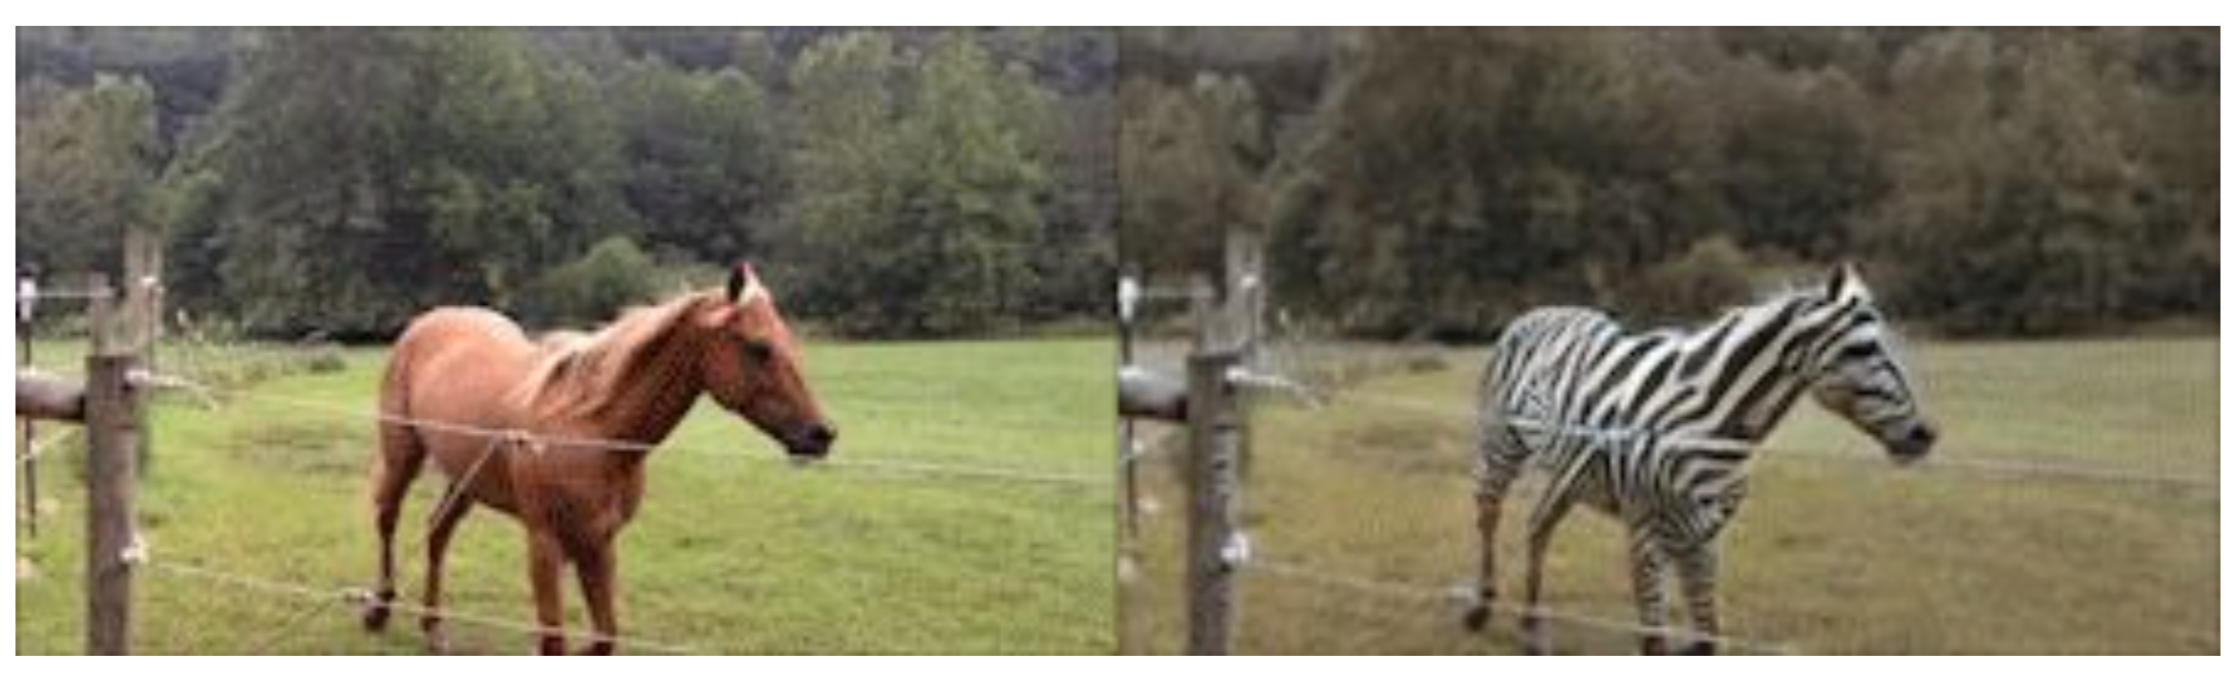
\includegraphics[width=1.0\linewidth]{figs/cyclegan.png}
        \label{fig:cyclegan}
    \end{figure}
\myfootnotewithlink{https://arxiv.org/abs/1703.10593}{Zhu J. Y. et al. Unpaired image-to-image translation using cycle-consistent adversarial networks, 2017}
\end{frame}
%=======
\begin{frame}{Applications: Face generation (StyleGAN)}
    \begin{figure}
        \centering
        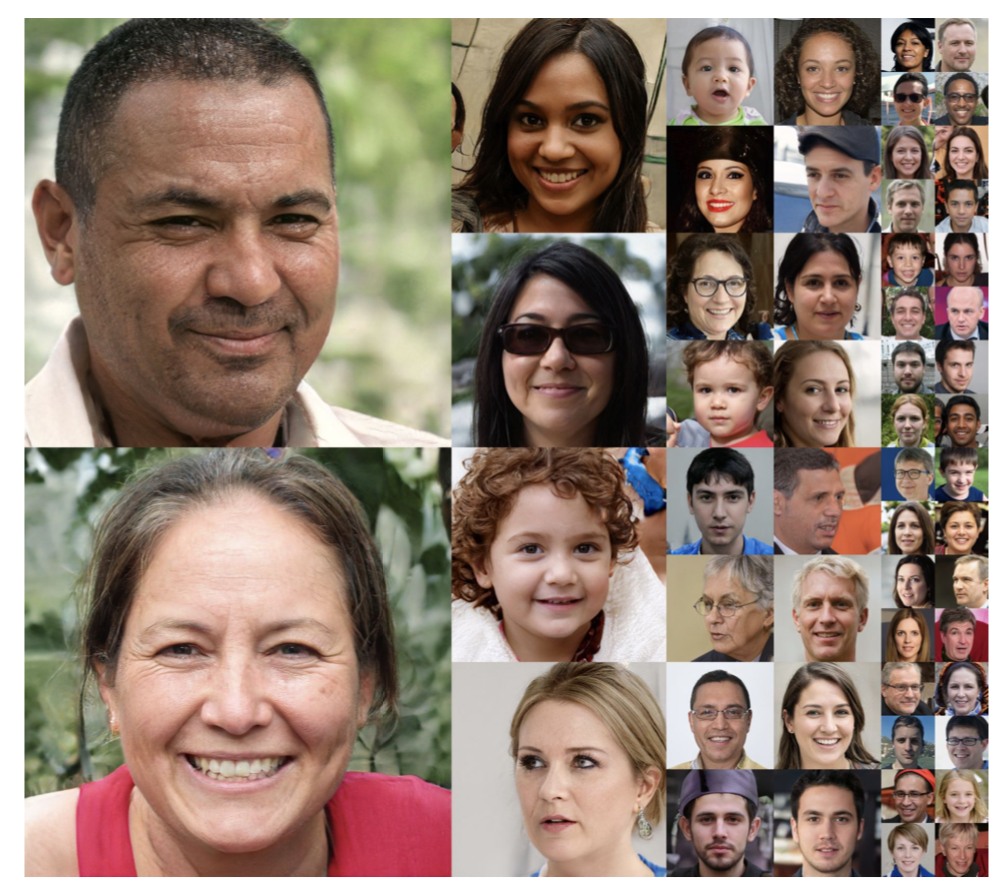
\includegraphics[width=0.65\linewidth]{figs/stylegan.png}
        \label{fig:stylegan}
    \end{figure}
\myfootnotewithlink{https://arxiv.org/abs/1812.04948}{Karras T., Laine S., Aila T. A style-based generator architecture for generative adversarial networks, 2018}
\end{frame}
%=======
\begin{frame}{Applications: Face generation (VQ-VAE-2)}
    \begin{figure}
        \centering
        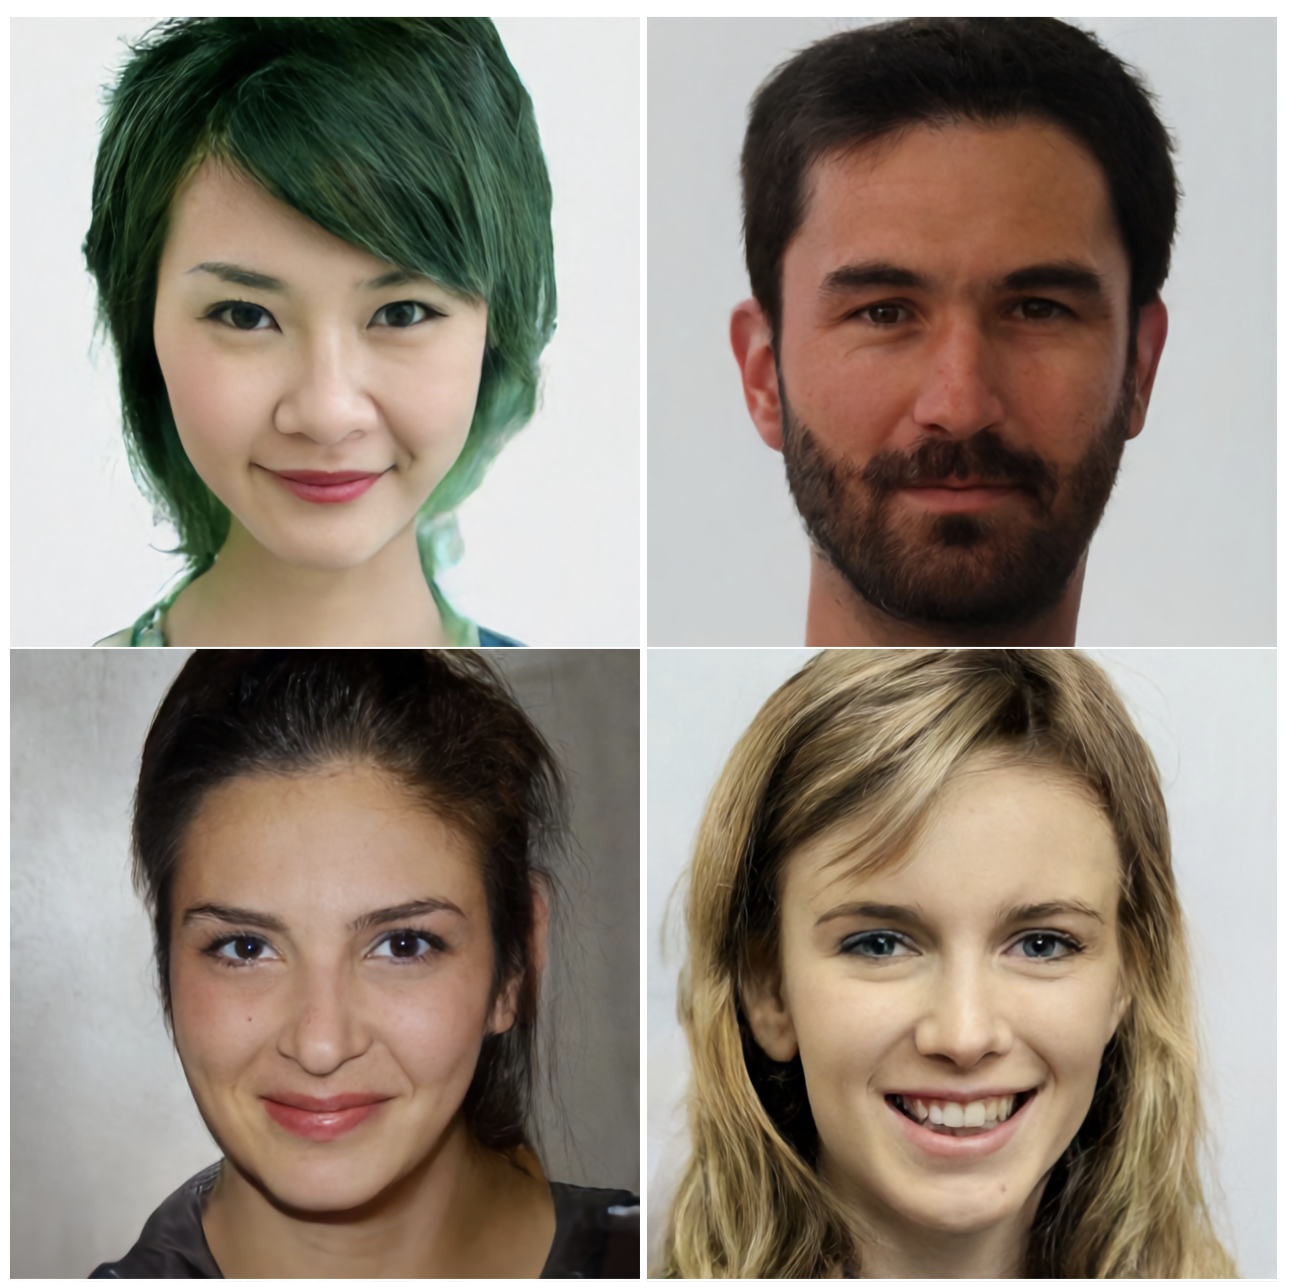
\includegraphics[width=0.65\linewidth]{figs/vq_vae.png}
        \label{fig:vq_vae}
    \end{figure}
\myfootnotewithlink{https://arxiv.org/abs/1906.00446}{Razavi A., Oord A., Vinyals O. Generating Diverse High-Fidelity Images with VQ-VAE-2, 2019}
\end{frame}
%=======
\begin{frame}{Applications}
\begin{itemize}
    \item Audio Generation (WaveNet, ...)
    \item Video Generation (DVD-GAN)
    \item NLP (Transformer, BERT, GPT-3, ...)
    \item Compression
\end{itemize}
\end{frame}
%--------------------------------------------------------------------------------
\section{Likelihood based models}
\begin{frame}{Problem Statement}
We are given samples $\{\bx_i\}_{i=1}^n \in X$ from unknown distribution $\pi(\bx)$.

\begin{block}{Goal}
	We would like to learn a distribution $\pi(\bx)$ for 
	\begin{itemize}
	    \item evaluating $\pi(\bx)$ for new samples;
	    \item sampling from $\pi(\bx)$.
	\end{itemize}
\end{block}
\begin{block}{Challenge}
	 Data is complex and high-dimensional (curse of dimensionality).
\end{block}
\end{frame}
%=======
\begin{frame}{Histogram as a generative model}

\begin{minipage}[t]{0.6\columnwidth}
    The histogram is totally defined by
	\[
	    p_k = p(x = k) = \frac{\sum_{i=1}^k [x_i = k]}{n}.
	\]
	\textbf{Problem:} curse of dimensionality. \\
	\vspace{0.05cm} \\
	MNIST: 28x28 gray-scaled images \\
	$2^{28\times28} - 1$ parameters to specify $p(\bx)$ 
	\end{minipage}%
	\begin{minipage}[t]{0.4\columnwidth}
    \begin{figure}[h]
        \centering
        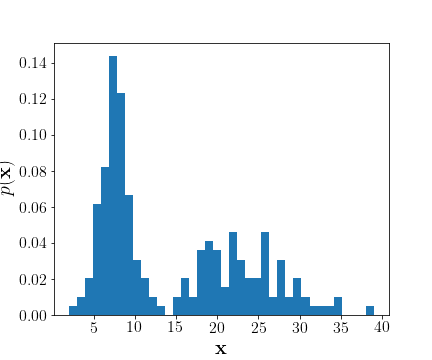
\includegraphics[width=\linewidth]{figs/histogram.png}
    \end{figure}
\end{minipage}
\[
    p(\bx) = p(x_1) \cdot p(x_2 | x_1) \cdot \dots \cdot p(x_m | x_{m-1}, \dots, x_1).
\]
\textbf{Question:} How many parameters do we need in these cases?
\[
    p(\bx) = p(x_1) \cdot p(x_2)\cdot \dots \cdot p(x_m).
\]
\[
    p(\bx) = p(x_1) \cdot p(x_2 | x_1) \cdot \dots \cdot p(x_m | x_{m-1}).
\]
\myfootnotewithlink{https://sites.google.com/view/berkeley-cs294-158-sp20/home}{image credit: https://sites.google.com/view/berkeley-cs294-158-sp20/home}
\end{frame}
%=======
\begin{frame}{Maximum likelihood}
    Fix probabilistic model $p(\bx | \btheta)$~-- the set of parameterized distributions . \\
    Instead of searching true $\pi(\bx)$ over all probability distributions, learn function approximation $p(\bx | \btheta) \approx \pi(\bx)$.
    
    \begin{block}{MLE problem}
    \vspace{-0.3cm}
    \[
        \btheta^* = \argmax_{\btheta} p(\bX | \btheta) = \argmax_{\btheta} \prod_{i=1}^n p(\bx_i | \btheta) = \argmax_{\btheta} \sum_{i=1}^n \log p(\bx_i | \btheta).
    \]
    \vspace{-0.1cm}
    \end{block}
    
    The problem is solved with SGD.
    \begin{block}{Requirements}
        \begin{itemize}
            \item efficiently compute $\log p(\bx | \btheta)$;
            \item efficiently compute gradient of $\log p(\bx | \btheta)$.
        \end{itemize}
    \end{block}
\end{frame}
\begin{frame}{Autoregressive model}
    \begin{block}{MLE problem}
    \vspace{-0.3cm}
    \[
        \btheta^* = \argmax_{\btheta} p(\bX | \btheta) = \argmax_{\btheta} \prod_{i=1}^n p(\bx_i | \btheta) = \argmax_{\btheta} \sum_{i=1}^n \log p(\bx_i | \btheta).
    \]
    \vspace{-0.1cm}
    \end{block}
    \begin{block}{Challenge}
    $p(\bx | \btheta)$ could be intractable.
    \end{block}
    \begin{block}{Likelihood as product of conditionals}
    Let $\bx = (x_1, \dots, x_m)$, $\bx_{1:i} = (x_1, \dots, x_i)$. Then 
    \[
        p(\bx | \btheta) = \prod_{i=1}^m p(x_i | \bx_{1:i - 1}, \btheta); \quad 
        \log p(\bx | \btheta) = \sum_{i=1}^m \log p(x_i | \bx_{1:i - 1}, \btheta).
    \]
    \end{block}
\end{frame}
%=======
\begin{frame}{Autoregressive models}
    \[
    \log p(\bx| \btheta) = \sum_{i=1}^m \log p(x_i | \bx_{1:i - 1}, \btheta)
    \]
    \begin{itemize}
        \item Each conditional could be modelled by neural network.
        \item To extend to high dimensions share parameters across conditionals.
        \item Sampling is sequential.
    \end{itemize}
    
\end{frame}
%=======
\begin{frame}{Char RNN}
	\begin{minipage}[t]{0.55\columnwidth}
		\begin{figure}[h]
			\centering
			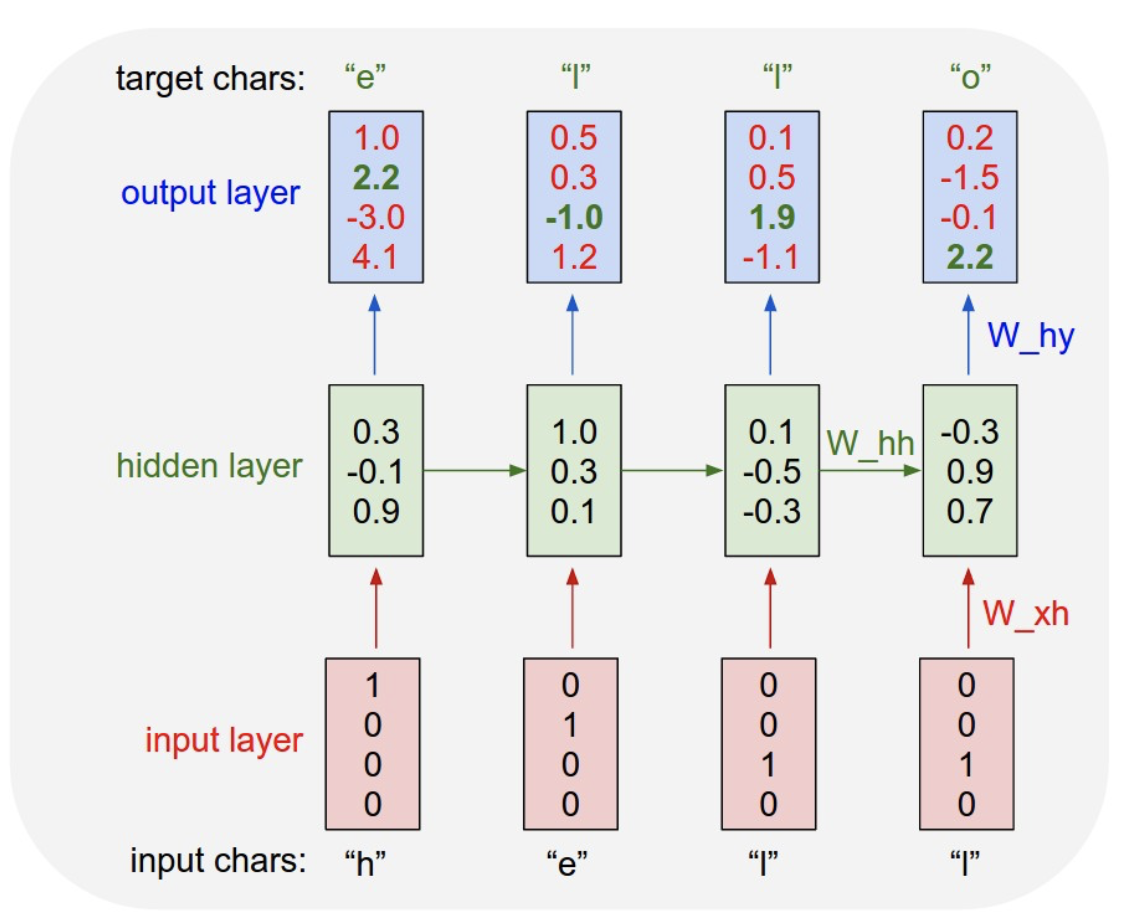
\includegraphics[width=1.0\linewidth]{figs/char_rnn.png}
		\end{figure}
	\end{minipage}%
	\begin{minipage}[t]{0.44\columnwidth}
		\begin{figure}[h]
			\centering
			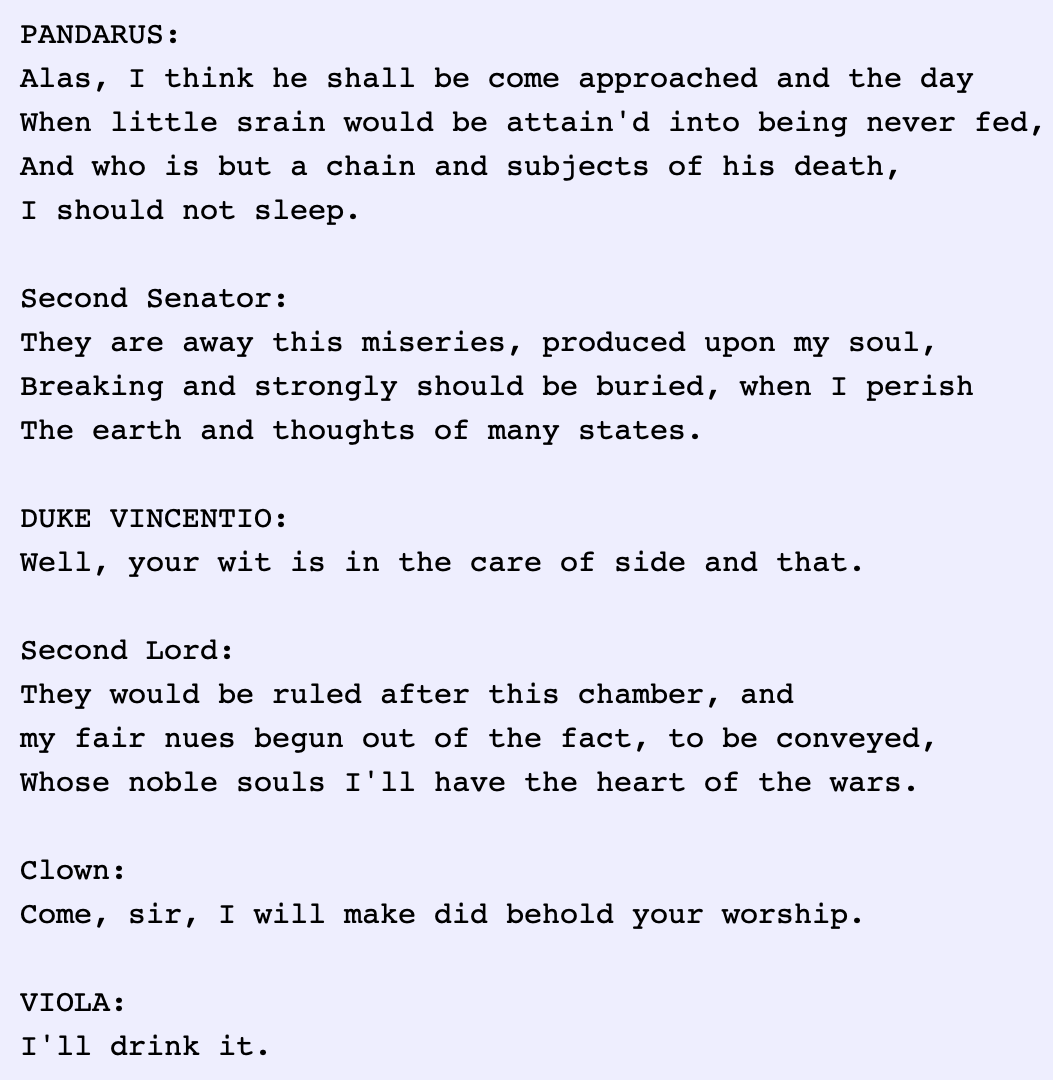
\includegraphics[width=1.0\linewidth]{figs/char_rnn_output.png}
		\end{figure}
	\end{minipage}
	\begin{block}{Drawback}
	Sequential computation of all conditionals $p(x_i | \bx_{1:i-1}, \btheta)$.
	\end{block}
\myfootnotewithlink{http://karpathy.github.io/2015/05/21/rnn-effectiveness/}{image credit: http://karpathy.github.io/2015/05/21/rnn-effectiveness}
\end{frame}
%=======
\begin{frame}{MADE}
\begin{figure}
    \centering
    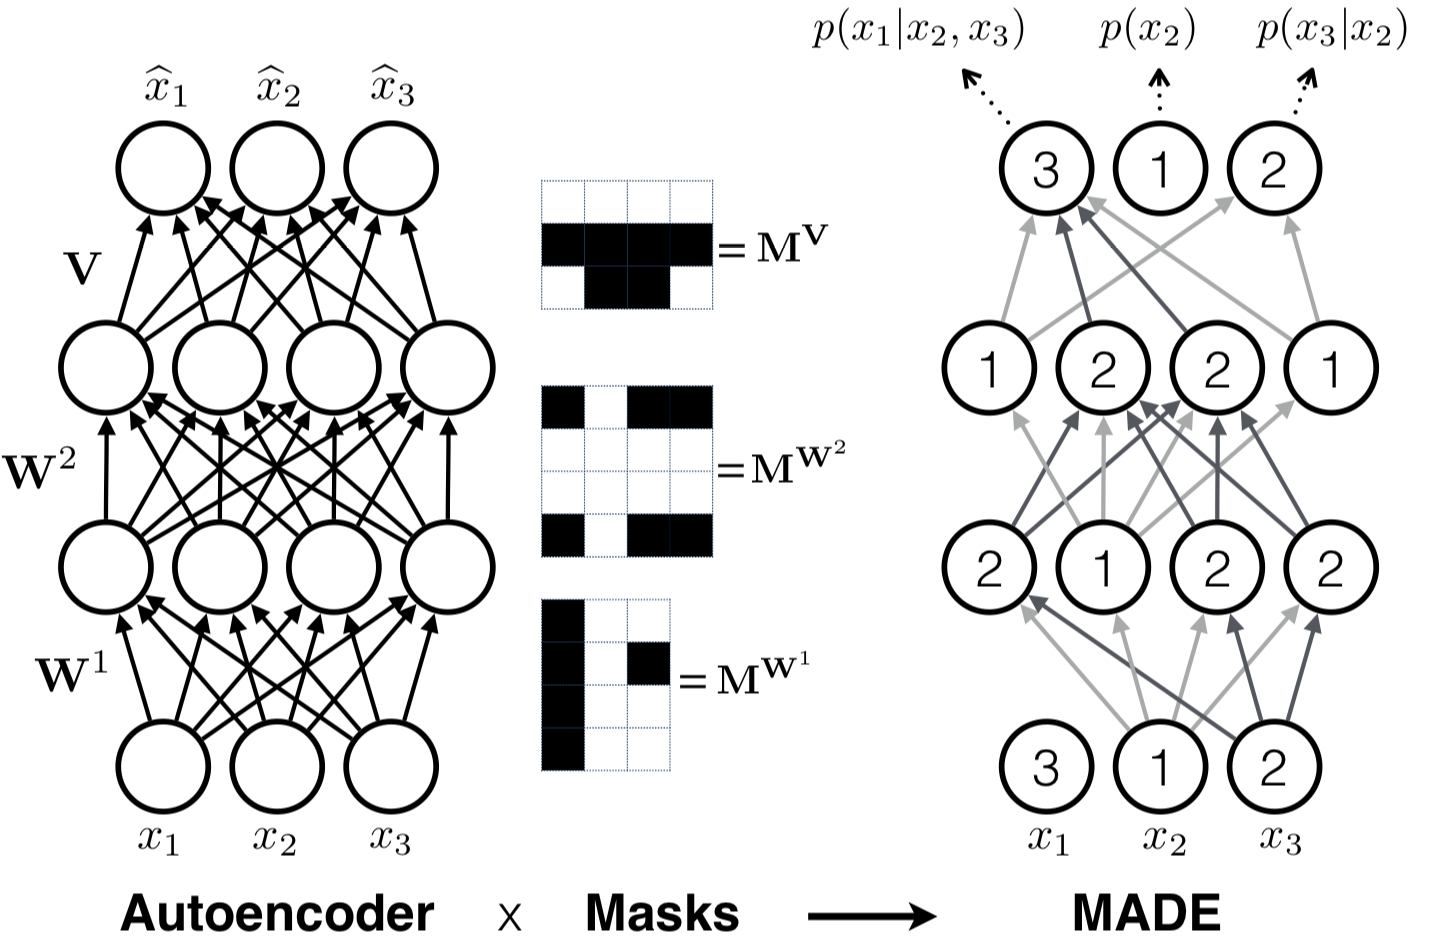
\includegraphics[width=0.9\linewidth]{figs/made.png}
    \label{fig:made}
\end{figure}
\myfootnotewithlink{https://arxiv.org/abs/1502.03509}{Germain M. et al. Made: Masked autoencoder for distribution estimation, 2015}
\end{frame}
%=======
%=======
\begin{frame}{WaveNet}
\begin{block}{Goal}
Efficient generation of raw audio waveforms with natural sounds.
\end{block}
\begin{block}{Solution}
Autoregressive model
\[
    p(\bx| \btheta) = \prod_{t=1}^T p(x_t|\bx_{1:t-1}, \btheta).
\]
\end{block}
The model uses causal dilated convolutions.
\begin{figure}
    \centering
    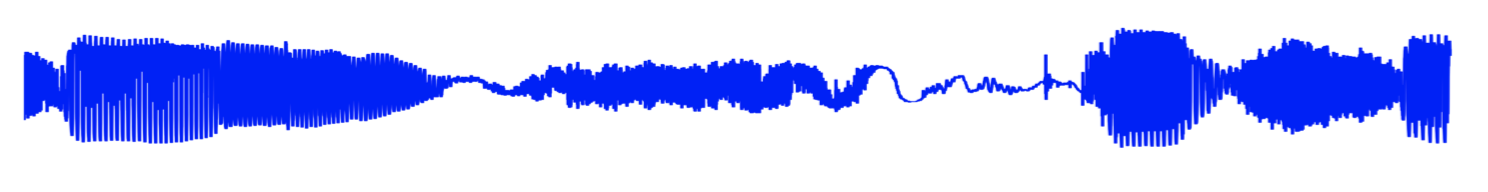
\includegraphics[width=0.9\linewidth]{figs/wavenet_ex.png}
\end{figure}
\myfootnotewithlink{https://arxiv.org/abs/1609.03499}{Oord A. et al. Wavenet: A generative model for raw audio, 2016}
\end{frame}
%=======
\begin{frame}{WaveNet (2016)}
\begin{figure}
    \centering
    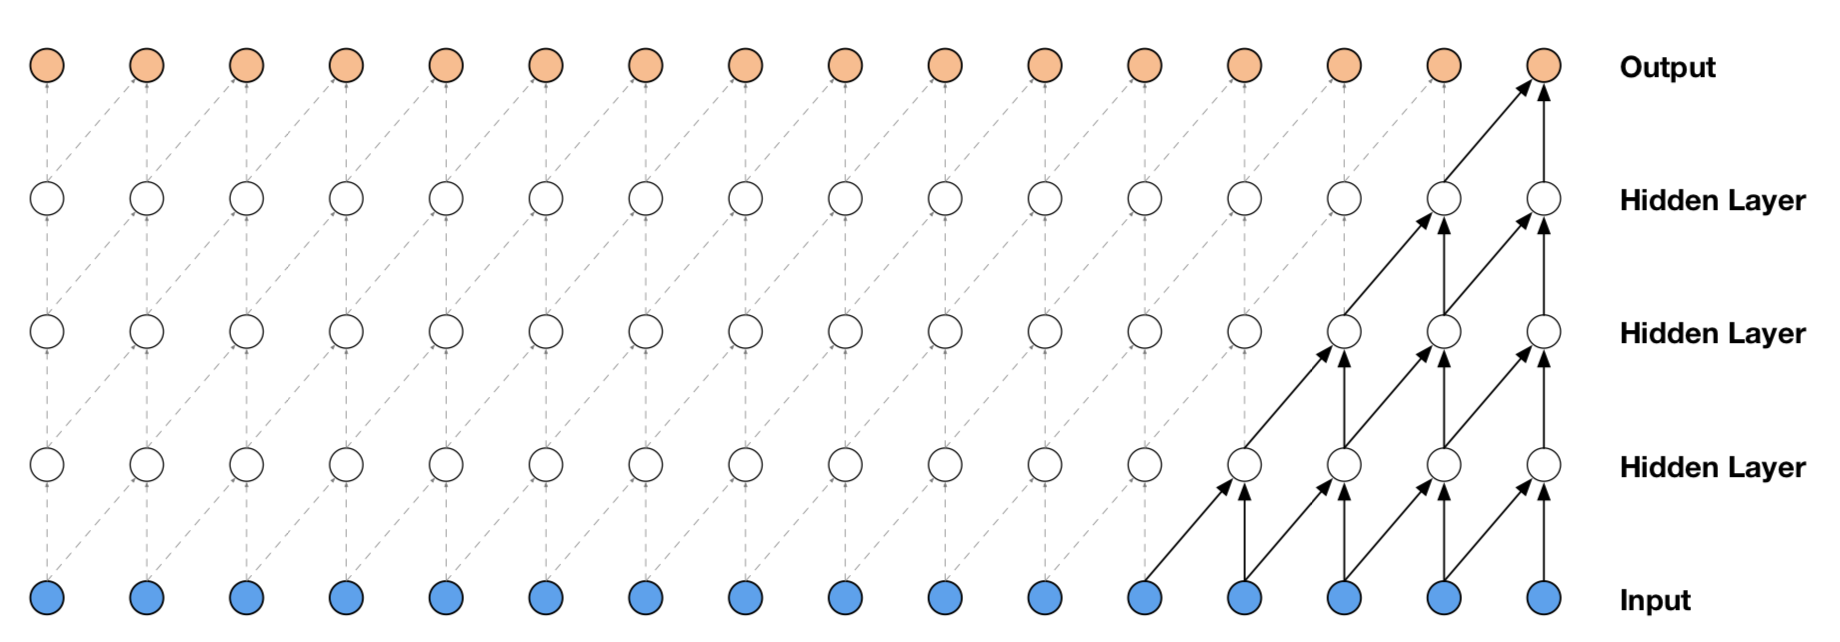
\includegraphics[width=0.9\linewidth]{figs/wavenet1.png}
\end{figure}

\begin{figure}
    \centering
    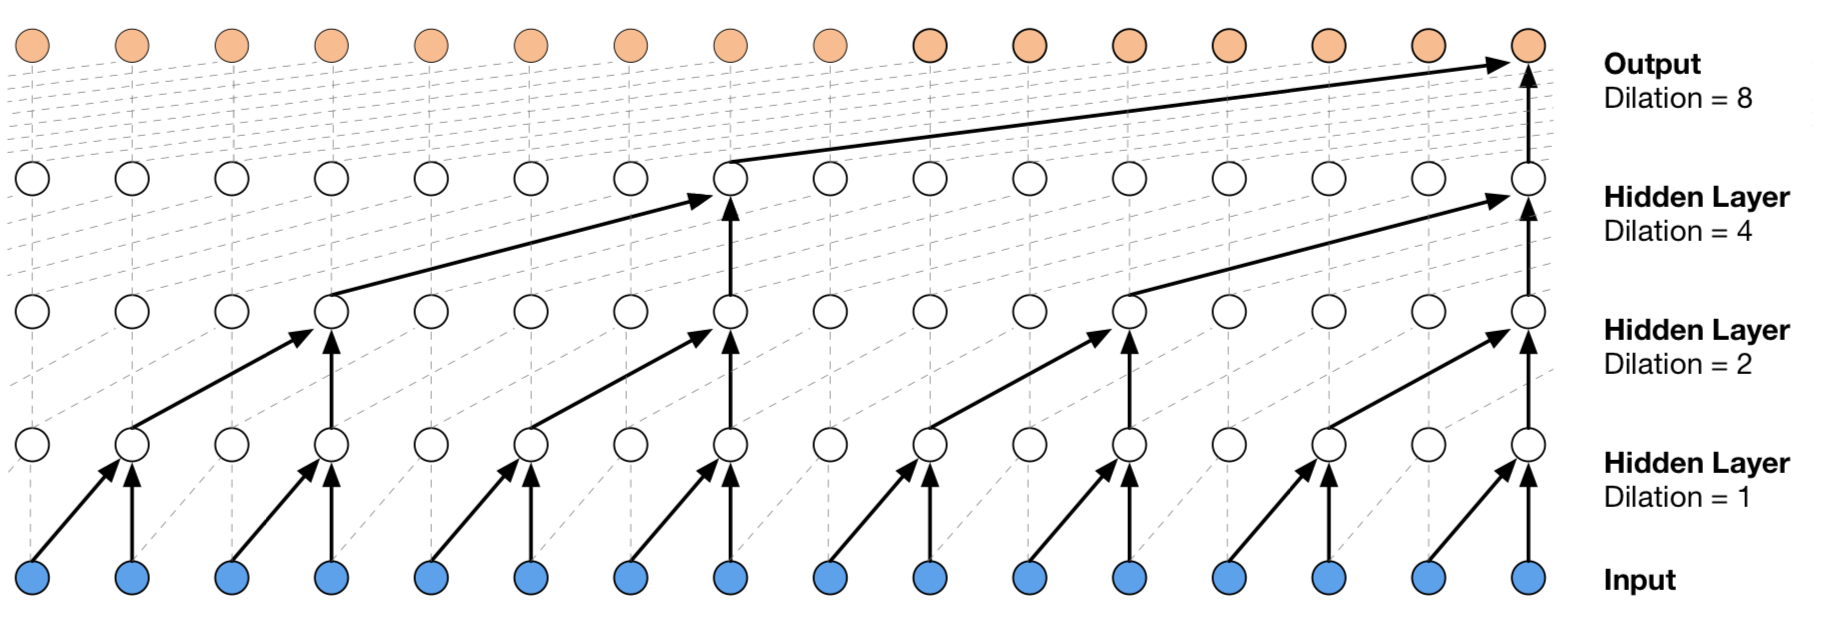
\includegraphics[width=0.9\linewidth]{figs/wavenet2.png}
\end{figure}
\myfootnotewithlink{https://arxiv.org/abs/1609.03499}{Oord A. et al. Wavenet: A generative model for raw audio, 2016}
\end{frame}

%=======
\begin{frame}{PixelCNN}
\begin{block}{Goal}
Model a distribution of natural images.
\end{block}
\begin{block}{Solution}
Autoregressive model
\[
    p(\bx | \btheta) = \prod_{i=1}^{n^2} p(x_i|\bx_{1:i-1}, \btheta).
\]
\begin{itemize}
    \item masked convolutions;
    \item dependencies over RGB channels.
\end{itemize}
\end{block}
\myfootnotewithlink{https://arxiv.org/abs/1601.06759}{Oord A., Kalchbrenner N., Kavukcuoglu K. Pixel recurrent neural networks, 2016}
\end{frame}
%=======
\begin{frame}{PixelCNN (2016)}
\begin{minipage}[t]{0.5\columnwidth}
	\begin{figure}[h]
		\centering
        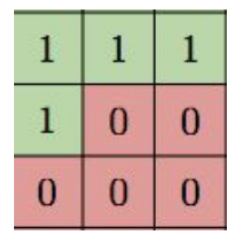
\includegraphics[width=0.35\linewidth]{figs/pixelcnn_0_1.png}
	\end{figure}
	\vspace{-0.1cm}
	\begin{figure}[h]
		\centering
        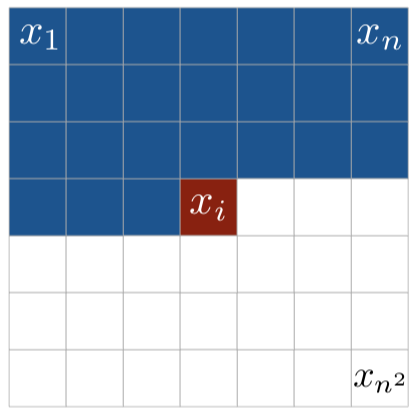
\includegraphics[width=0.7\linewidth]{figs/pixelcnn1.png}
	\end{figure}
	\end{minipage}%
	\begin{minipage}[t]{0.5\columnwidth}
	\begin{figure}[h]
		\centering
        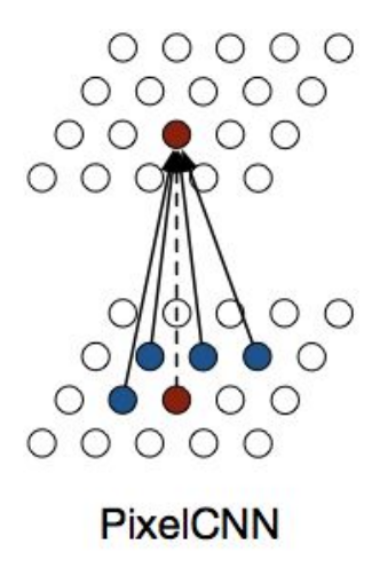
\includegraphics[width=0.5\linewidth]{figs/pixelcnn_0_2.png}
	\end{figure}
	\vspace{-0.4cm}
	\begin{figure}
		\centering
        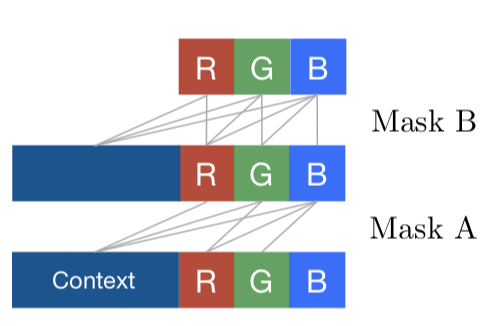
\includegraphics[width=0.65\linewidth]{figs/pixelcnn2.png}
	\end{figure}
\end{minipage}
\myfootnotewithlink{https://arxiv.org/abs/1601.06759}{Oord A., Kalchbrenner N., Kavukcuoglu K. Pixel recurrent neural networks, 2016}
\end{frame}
%=======
\begin{frame}{Summary}
    \begin{itemize}
        \item Sampling from autoregressive models is trivial, but sequential
        \begin{itemize}
            \item sample $x_0 \sim p(x_0)$;
            \item sample $x_1 \sim p(x_1 | x_0)$;
            \item \dots.
        \end{itemize}
        \item Estimating probability:
        \[
            p(\bx) = \prod_{i=1}^m p(x_i | \bx_{1:i - 1}).
        \]
        \item Work on both continuous and discrete data.
        \item There is no natural way to do unsupervised learning.
    \end{itemize}
\end{frame}
%=======
\begin{frame}{Summary}
\end{frame}

\end{document} 